\pagebreak
\section{Field Deployment at\\Tungurahua Volcano}
\label{sec-deploy}
\label{sec-deployment}

To evaluate the performance of Lance in a real field setting, 
we undertook a one week deployment of eight~sensor nodes at
Tungurahua Volcano, Ecuador, in August~2007. Lance was used to manage
the bandwidth resources of the sensor network, as
described below. Time and budget constraints prevented us from deploying 
a larger network for longer period of time. 
An earlier version of Lance was used in this deployment
that did not explicitly model energy cost in the download manager. 
However, due to the short duration of the deployment, we knew that 
the battery lifetime used would be more than adequate (two D-cell batteries
offer a lifetime of approximately 12~days with this platform). 
Our primary goal was to validate Lance's operation in a field campaign, 
as well as to identify challenges that only arise in real deployments.

\begin{figure}[t]
\begin{center}
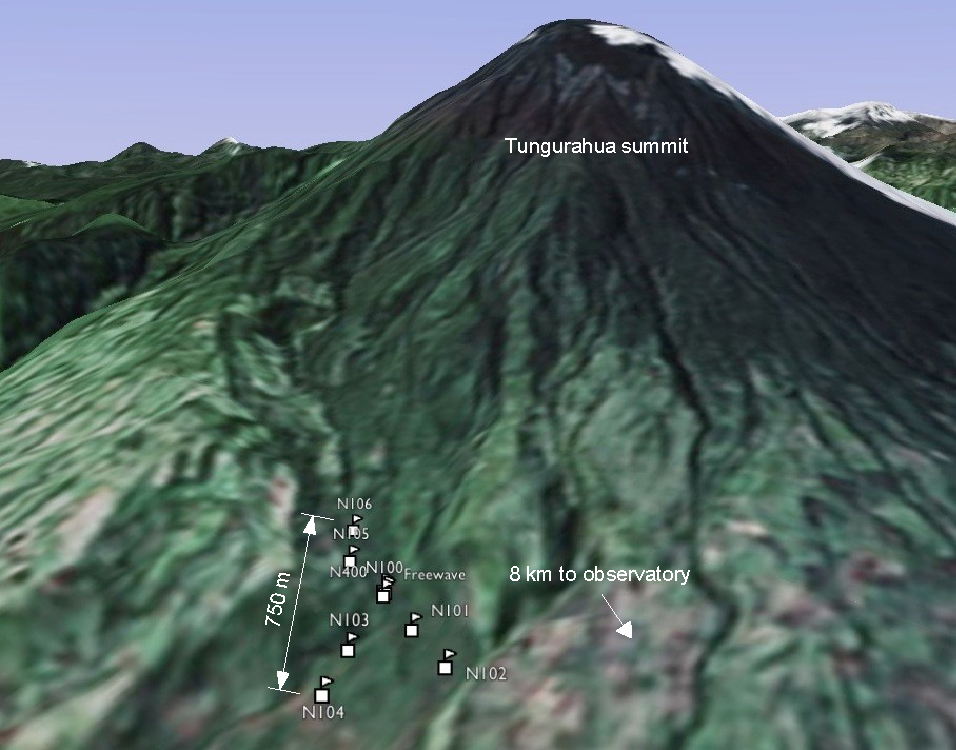
\includegraphics[width=1.0\hsize]{./lance/figs/deploy/deployment-map.pdf}
\end{center}
\caption{\small {\bf Location of the Tungurahua sensor network
deployment.}}
\label{fig-deploy-map}
\end{figure}

The hardware design was based on one used in a previous volcano sensor
network deployment~\cite{volcano-osdi06}.
Each sensor node consisted of a TMote~Sky module
coupled with a custom 24-bit multichannel~ADC board. The network measured
seismic signals using 4.5~Hz geophones and infrasonic signals with small
electret microphones attached to each node.  Data was sampled at 100~Hz
per channel. As shown in Figure~\ref{fig-deploy-map}, seven of the nodes 
were deployed in a three-armed ``star'' topology radiating away from 
a central hub node, with two nodes per arm. 
The eighth node was colocated with the hub and 
transmitted an unreliable continuous stream of sensor data packets 
for establishing ground truth. 
A separate gateway node relayed data (using a FreeWave radio modem) 
to the base station laptop at the volcano observatory, 8~km
from the deployment site. Time synchronization was established using
FTSP~\cite{ftsp} with a single GPS receiver as the root of the
synchronization tree. 
We experimented with two different summarization functions as well as
several different policy modules during the field deployment.

\subsection{Overall performance and data yield}

% Yield: How much data did we download during the deployment? How was it
% distributed across nodes?

% First download log: 2007-08-02T15:14:00.70Z
% Last download log: 2007-08-04T23:58:48.192Z
% Total time for downloads: 56 hours
% First streamutility log: 2007-08-02T15:14:00.55Z
% Last streamutility log: 2007-08-05T14:51:00.232Z
% Total time for deployment: 71 hours

% Data here comes from running "DownloadStats.py" on all of the
% data/generated/gps-DownloadManager-08-0[2345]*
\begin{figure}[t]
\begin{center}
\begin{small}
\begin{tabular}{|l|l|l|} \hline 
{\bf Node}	& {\bf ADUs downloaded} & {\bf Mean throughput} \\ \hline
100 & 311 & 651.0 B/sec \\
101 & 131 & 446.8 B/sec \\
102 & 262 & 445.8 B/sec \\
103 & 292 & 424.4 B/sec \\
104 & 150 & 256.8 B/sec \\
105 & 66 & 453.7 B/sec \\
106 & 20 & 253.4 B/sec \\ \hline
{\em Total} & 1232 & 431.5 B/sec \\ \hline
\end{tabular}
\end{small}
\end{center}
\caption{\small {\bf Download performance during the deployment.}}
\label{fig-deploy-throughput}
\end{figure}

The sensor network was operational for a total of 71~hours, out of
which the Lance download manager ran for a total of 56~hours. 
During this time, Lance successfully downloaded 1232~ADUs, or 77~MB of 
raw data. An additional 308~downloads failed due to timeout or stale summary 
information, for an overall success rate of 80\%. 
% Number below obtained by running SimulateLance.py on all of the
% LogUtility logs during the deployment, reading in all of the
% utility summaries but screening out those with bogus 65534 values.
11012~unique ADU summaries were received from the network,
representing an aggregate of 688~MB of sampled data. Lance therefore
downloaded approximately 11\% of the data produced by the network.
% Performance: What was the overall fetch throughput? Distribution of 
% fetch times?
Figure~\ref{fig-deploy-throughput} summarizes the number of ADUs
downloaded and the mean throughput for each node. 

% Overheads

\begin{figure}[t]
\begin{center}
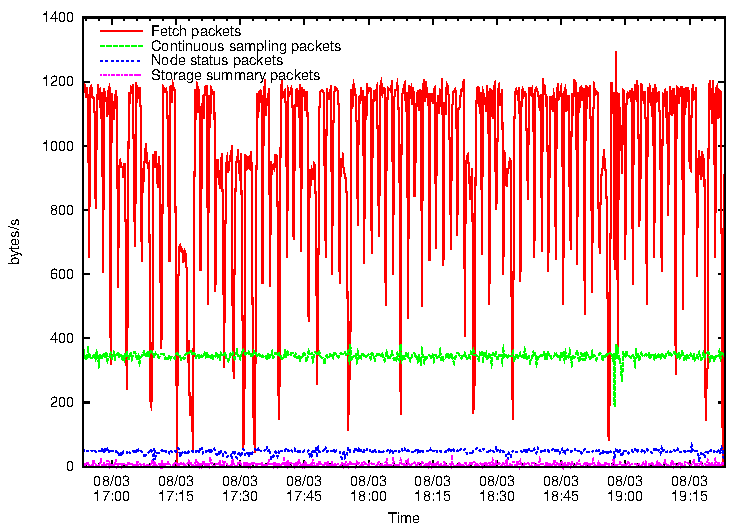
\includegraphics[width=0.9\hsize]{./lance/figs/deploy/packetgraph/packetgraph.pdf}
\end{center}
\caption{\small {\bf Breakdown of radio traffic by packet type.}
{\em This figure shows the total number of bytes received at the base 
station, averaged over 15~sec intervals. Periodic node status messages
and storage summaries comprise a small fraction of the overall
bandwidth.}}
\label{fig-packetgraph}
\end{figure}

Figure~\ref{fig-packetgraph} shows a breakdown of the packets received
at the base station for a representative time period.
Fetch download packets consumed the majority of
the bandwidth, followed by the continuous sampling packets.
The latter is a debugging feature allowing us to visualize the
seismic activity from a single node in real time, and is entirely optional.
Every node sent a periodic heartbeat to the base station every~10~sec,
and a storage summary every 109~sec. As the figure shows, this
overhead is a small percentage (less than 5\%) of the overall network
traffic. 

% From Steve:
% Type			Num packets 	Size	Total bytes
% ReplyMsg		193637  	58	11230946 (4.21%)
% ContinuousSamplingMsg	1325069 	51	67578519 (25.36%)
% FetchReply 		3592552 	51	183220152 (68.77%)
% GPSReceiver		27793   	27	750411
% TimeSync		117774  	16	1884384
% UtilityStreamer	34423		51	1755573 (0.65%)
% Total						266419985

\pagebreak
\subsection{RSAM-based summarization}

\begin{figure}[t]
\begin{center}
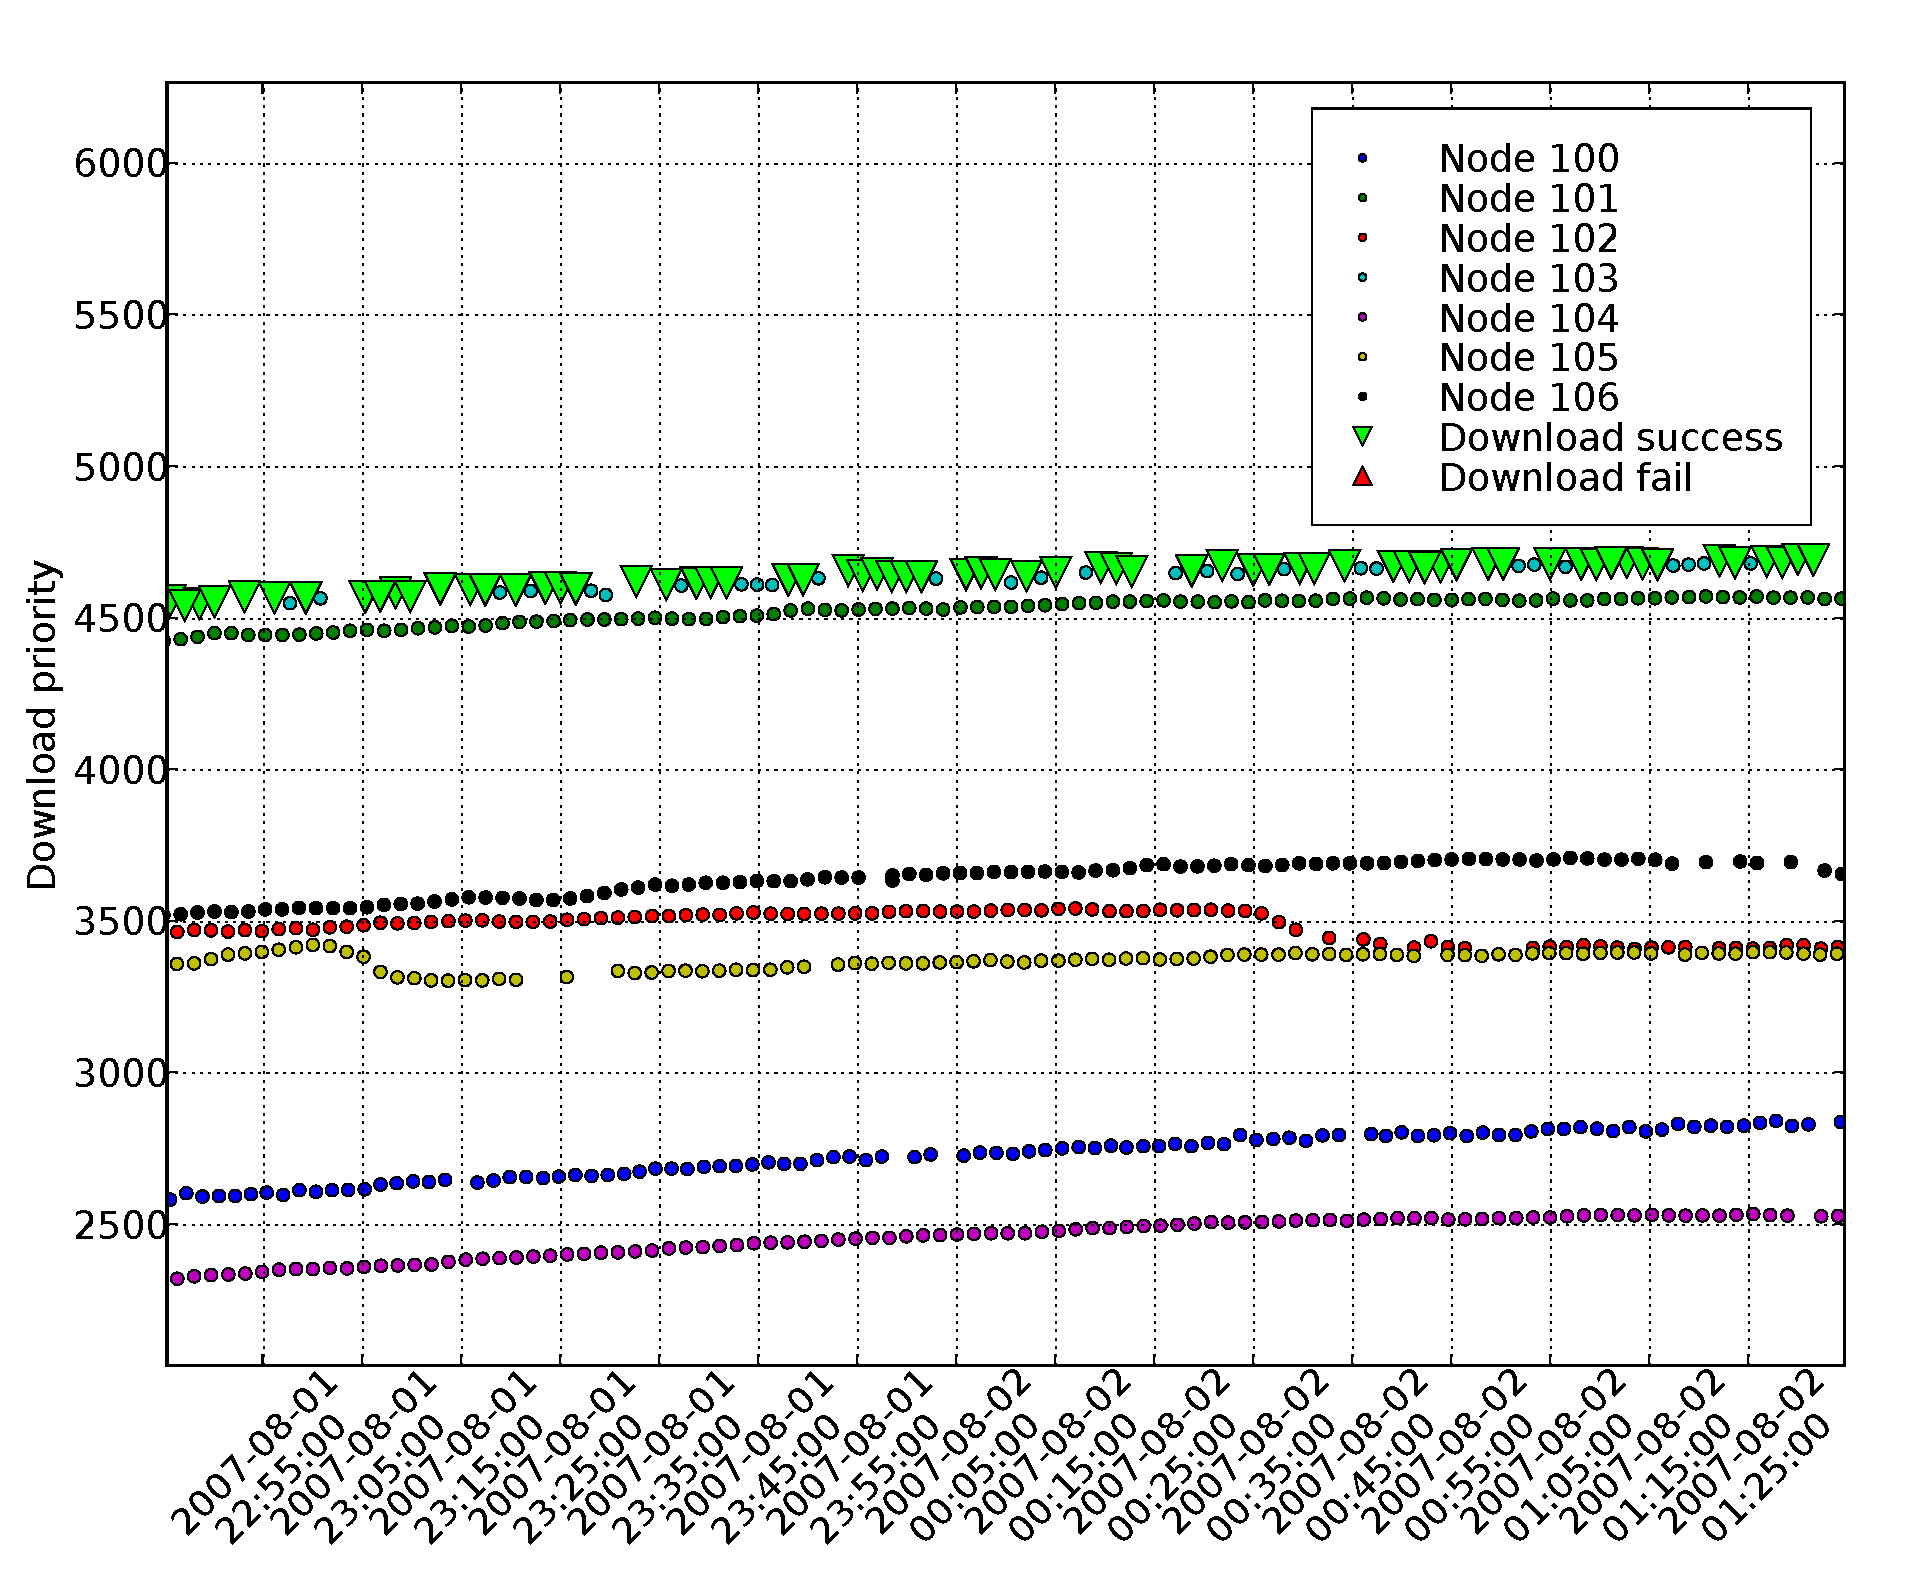
\includegraphics[width=1.0\hsize]{./lance/figs/deploy/downloads-pre-median-filter5.pdf}
\end{center}
\caption{\small {\bf Effect of DC bias on RSAM summarization
function.} {\em Each point represents the ADU value received at
the base station, and the triangles indicate those ADUs that were
downloaded by Lance. Since nodes' RSAM values are
offset significantly from each other, Lance prefers
downloading from the node with the largest positive bias.}}
\label{fig-rsam-dc-bias}
\end{figure}

The system as initially deployed computed the RSAM~\cite{rsam} as the
value for each ADU.
This approach was intended to prioritize data based on
the overall level of seismic activity. We experienced two problems as
soon as the system was fielded. First, the RSAM calculation was
sensitive to DC~bias in the seismometer signal, causing Lance to 
generally prefer downloading ADUs from one or two nodes (those with
the largest positive bias). Figure~\ref{fig-rsam-dc-bias} shows this
effect, with Lance only downloading ADUs from node~103.

This problem was easily corrected, without any node software changes,
by introducing a policy module at the base station to process the 
raw RSAM values received
from each node and filter out the DC~bias. This was achieved by
computing the median RSAM value over each 30-minute window of raw RSAM
values on each node, and subtracting the median from the RSAM.

The second problem with the RSAM summarization function was caused
by the uncharacteristically low level of seismicity at the volcano
throughout the deployment. We observed only about 20~volcano-tectonic 
earthquakes and {\em no} clear explosions, whereas the previous week,
Tungurahua exhibited dozens of earthquakes each day. As a result, the
RSAM summarization function was generally unable to distinguish between
actual seismic activity and noise. We corrected this problem by
switching to a different summarization function (described below)
that was designed to pick out small earthquakes. 

% MDW: These results are based on running SimulateLance.py.  Note that
% "optimal" here is actually the top K ADUs bounded by the duration to
% download them, NOT the knapsack solution (which takes forever to run.)
To evaluate Lance's behavior with respect to an ``optimal'' system, we took
the 8483~RSAM summaries received during a 16-hour period when the debiasing
filter was enabled. Using this information, we compute the set of ADUs that
the optimal system would have downloaded, with complete knowledge of all ADUs
but limited to the same time duration the original network was operating.  We
assume the download throughput for a given node is always the mean throughput
for that node observed during the deployment
  (Figure~\ref{fig-deploy-throughput}). This calculation ignores energy
  constraints because the deployed system did not consider energy costs.

% Optimal: 392 downloads, utility 10678
% Actual: 419 downloads, utility 10629
% Noflash: 351 downloads, utility 10030
% Flash: 371 downloads, utility 9440
% Fifo: 339 downloads, utility 6633 

An optimal system would have downloaded 392~out of the~8483 ADUs,
whereas the actual system downloaded 418~ADUs during this 
time.\footnote{The optimal system would download fewer ADUs 
than the real system due to the variation in the throughput to each 
node: the optimal system would download more ADUs from nodes 
with lower throughput, thereby limiting the total number of ADUs it could
download.} The total value of ADUs downloaded by the optimal system 
is 10678, whereas the value of the actual network was 10629, for an
optimality of 99.5\%. Lance did an exceptional job of extracting the
highest-value data from the network using our online heuristic
algorithm.

%We can also ask how much overlap there is between the actual
%downloaded ADUs and those downloaded by the optimal system. 
%In this case, 235 out of the 392~``optimal'' ADUs were downloaded by
%the real network, yielding an overlap of 60\%. Although the
%two systems chose different particular ADUs to download, the aggregate
%utility of the two data sets are very similar. 

% RSAM: Explain DC bias problem and show it. Explain how we fixed it
% with the median filter policy module. 

% Distribution of RSAM values
% Distribution of RSAM values for data successfully downloaded.

% Say we could have stored all of the data in the network forever (no 
% storage expiration). Given a limit on download throughput how well
% did we do in terms of capturing the "highest utility" ADUs? That is,
% rank order all of the ADUs according to utility value and assume a
% certain overall download rate from the network: take a 24-hour
% period and ask how much data we can download during that time, then
% see how that compares to the ADUs actually downloaded. 
%   - Similar to the evaluation that GWA is doing I believe.

% -----
\subsection{EWMA-based summarization function}
\label{sec-ewma-deployment}

Given the low level of volcanic activity, after the first 25~hours of
the deployment we chose to reprogram the network to use a different
summarization function that is designed to pick out small earthquakes
from background noise. This function computes the maximum ratio of two
EWMA filters over the seismic signal; it is similar to that described
in~\cite{volcano-osdi06}. Due to code size limitations on
the motes, it was necessary to manually reprogram each node with the
new summarization function, which took two teams about 4~hours.

% EWMA: Big problem here is that we trigger an ADU regardless of where
% in the ADU the event occurs. As a result we may miss the head or
% tail of the event if it occurs near the beginning or end of the ADU.

This summarization function reports a high value for an ADU
that appears to contain an earthquake or other seismic event. 
However, there is no guarantee that the event will be centered in the
ADU: in the worst case, the earthquake might occur at the very
beginning or very end of the ADU, causing the initial seismic P-wave arrival
or waveform coda to be stored in adjacent ADUs with low value.
To avoid this problem, we made use of the {\tt timespread} policy
module that detects ADUs with
an elevated value (over a fixed threshold) and assigns the
immediately preceding and succeeding ADUs the same value.
By dilating the value over time, Lance should download
all three of the ADUs and maximize the probability that a given
earthquake signal is entirely downloaded.

% optimal: Total downloads: 554, utility 577377
% actual: Total downloads: 518, utility 539115
% noflash: Total downloads: 470, utility 490069
% flash: Total downloads: 454, utility 473086
% fifo: Total downloads: 470, utility 488119

As with the RSAM-based summarization function, we estimate the optimal set of
ADUs that an oracle would have downloaded. During a 25-hour period, the
network reported 11012~unique ADU summaries. An optimal system would have
downloaded 554 ADUs with total value 577377.  The actual network
downloaded 518~ADUs with a value of 539115, for an optimality of 93.3\%. 

% Idea: Take 'ground truth' data and window each 'event' with a 60-sec
% window. Look at the data we actually downloaded from the network
% and see how much overlap there is. 

As a final evaluation metric, we wish to consider how well Lance,
configured in this manner, was able to download seismic signals
representing earthquakes. Given the low level of volcanic activity, 
it turns out that most of the ADUs downloaded by Lance contain no 
discernible seismic signal. In fact, upon manual inspection of the
518~ADUs downloaded during this period, we identified only 20~ADUs
showing a clear earthquake signal, corresponding to only 9~separate
seismic events.\footnote{One seismologist remarked that we 
``fixed the volcano'' by placing our sensors on it.}
Note that we did {\em not} configure Lance to explicitly download 
correlated earthquakes as described in Section~\ref{sec-applications},
so we would not expect a high degree of coverage for the same event
across multiple nodes.

\begin{figure}[t]
\begin{center}
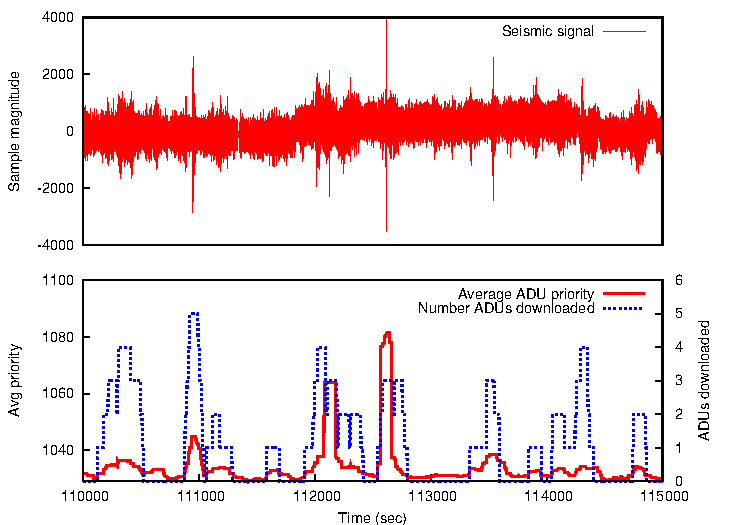
\includegraphics[width=1.0\hsize]{./lance/figs/deploy/deploydownloads/everything.pdf}
\end{center}
\caption{\small {\bf Lance download behavior overlayed with average
ADU value.} {\em The top plot shows the continuous seismic signal
collected by a single node. The lower plot shows the average value
of ADUs and the number of ADUs downloaded for each window.}}
\label{fig-downloads-cont}
\end{figure}

Figure~\ref{fig-downloads-cont} shows the behavior of Lance during a
representative 83-minute period. In the figure, we have broken time
into windows of one-half an ADU duration (55~sec in this case), and
computed the mean ADU value as well as the number of downloaded
ADUs that overlap each time window. As the data shows, elevated seismic
activity is well-correlated with an increase in the ADU value
from across the network, as well as the number of downloaded ADUs.
Moreover, the few cases of clear seismic activity in the trace 
(at times 111000, 112700, and so forth) tend to have more ADUs
downloaded. Of the 9~separate seismic events, a total of 27~ADUs were
downloaded, representing a per-event ``coverage'' of 3~ADUs per event.
This represents just under half of the 7~nodes participating in the network.

%To verify that is the case, we manually reviewed each of the 518 ADUs
%downloaded during this period, and marked those which contained interesting
%events. Of these segments, we found only 20~ ADUs which contained clear signs 
%of volcanic activity. 
%For each ADU, we computed the set of overlapping
%ADUs downloaded from other nodes that overlap by at least one half of
%an ADU time (55~sec in this case). 

%For our
%analysis, we chose two window sizes, half the length of one ADU (about 55
%seconds).  Using this information, we considered two manually-marked events in
%our downloaded ADUs to be part of the same volcanic event if they both appear
%in one of these sets.

%Using a window size equal to half the length of an ADU, the 20 manually marked
%ADUs reduced to only nine distinct volcanic events.  Additionally, by looking
%at other ADUs downloaded that we did not manually mark, yet still overlapped,
%we found a total of 27 ADUs within our window of a marked event.  Thus, for a
%detected event during the period where we ran the EWMA summarizer, we
%downloaded an average of three separate ADUs covering that event.

%\begin{table}[htbp!]
%\begin{center}
%\begin{small}
%\begin{tabular}{|l|l|l|} \hline 
%Total downloaded ADUs         & 518 \\
%Hand-marked events            & 20  \\
%Non-overlapping events        & 9   \\
%Total downloaded volumes covering events & 27 \\
%Average coverage              & 3 ADUs \\
%\hline
%\end{tabular}
%\end{small}
%\end{center}
%\caption{\small {\bf Coverage of volcanic events while using EWMA}.  The
%  window used was $\frac{1}{2}$ the length of an ADU.}
%\end{table}

